\documentclass[a4paper,12pt]{article}
\usepackage{float}
\usepackage[table]{xcolor} % Para colorir as linhas da tabela
\usepackage{array} % Para melhorar a formatação de tabelas
\usepackage[brazil]{babel}
\usepackage[utf8]{inputenc}
\usepackage{indentfirst}
\usepackage{amsmath}
\usepackage{multicol}
\usepackage{graphicx}
\usepackage{animate}
\usepackage{tabularx}
\usepackage[font=footnotesize, labelfont=bf, listformat=empty]{caption}
\usepackage{geometry}
\usepackage{listings}
\usepackage{lastpage}
\usepackage{subcaption}
\usepackage[skins,xparse,breakable]{tcolorbox}
\usepackage{longtable}
\usepackage{minted}
\usepackage{titlesec}
\usepackage{fancyhdr}
\usepackage{setspace}
\usepackage[colorlinks=true, allcolors=black]{hyperref}

\usetikzlibrary{arrows,shapes,automata,positioning,calc}
% Configurações de margens e espaçamento
\geometry{a4paper, left=2.5cm, right=2.5cm, top=2.5cm, bottom=2cm}
\onehalfspacing

% Configurações de títulos
\titleformat{\section}{\normalfont\large\bfseries}{\thesection}{1em}{}
\titleformat{\subsection}{\normalfont\bfseries}{\thesubsection}{1em}{}
\titleformat{\subsubsection}{\normalfont\itshape}{\thesubsubsection}{1em}{}

% Configurações de listagens
\renewcommand{\listingscaption}{Código}
\newenvironment{code}{\captionsetup{type=listing}}{}

% Configurações de cores
\definecolor{LightSeaGreen}{rgb}{0.1255, 0.6980, 0.6667}
\definecolor{whitesmoke}{rgb}{0.96, 0.96, 0.96}
\definecolor{cinza}{RGB}{160, 160, 160}
\definecolor{cinza_claro}{RGB}{240, 240, 240} % Cinza claro

% Configurações do minted para VHDL
\setminted[VHDL]{
    fontsize=\footnotesize,
    style=emacs,
    linenos=true,
    breaklines=true,
    mathescape=true,
    bgcolor=cinza_claro,
    breakanywhere=true,
}

\tikzset{
    state/.style={
        circle,
        thick,
        draw=black!100,
        fill=white!100,
        minimum size=12mm,
        align=center
    },
    accepting/.style={
        double,
        double distance=1.2pt
    }
}

\newcommand{\hex}[1]{\textcolor{green!50!black}{#1}}

% Configurações de cabeçalho e rodapé
\pagestyle{fancy}
\fancyhf{}
\fancyhead[L]{\footnotesize{Laboratório de Sistemas Digitais - ENE0040}}
\fancyhead[R]{\footnotesize{2025/1 - Turma 07}}
\fancyfoot[R]{\footnotesize{Página \hspace{0.05cm} \thepage \hspace{0.05cm} de \pageref{LastPage}}}
\fancyfoot[L]{\footnotesize{Relatório do Experimento 7}}

% Adiciona uma linha preta acima do rodapé
\renewcommand{\footrulewidth}{0.4pt} % Espessura da linha
\renewcommand{\footrule}{\vbox to 0pt{\hrule width \textwidth height \footrulewidth \vss}} % Desenha a linha

% Novo Comando para chamar a capa
\newcommand{\capa}{
    \begin{titlepage}
        \begin{multicols}{2}
            \begin{flushleft}
                
\includegraphics[width=0.45\linewidth]{Recursos/Imagens/UnB_logo.png}
            \end{flushleft}
            \columnbreak
            \begin{flushright}
                Universidade de Brasília \\
                Faculdade de Tecnologia \\
                Departamento de Engenharia Elétrica
            \end{flushright}
        \end{multicols}
        \begin{center}
        \vspace{-20pt}
        \rule{\textwidth}{0.4pt}
        \end{center}
        \vspace{0.6cm}
        \begin{center}
            {\Huge \textbf{Relatório do Experimento 7}} \\[1em]
            {\large \textbf{Autor:} Henrique Morcelles Salum} \\[0.5em]
            {\large \textbf{Matrícula:} 232003008} \\
            \vfill
            {\large \textbf{ENE0040 - Laboratório de Sistemas Digitais - Turma 07}} \\
        \end{center}
    \end{titlepage}
}

\begin{document}

\capa

% Sumário
\newpage
\tableofcontents
\newpage

% Introdução
\section{Introdução}

Este experimento é composto de apenas uma tarefa: implementar um moedeiro por meio de uma máquina de estados finita. Esse moedeiro é utilizado no contexto de uma máquina de refrigerantes simplificada, que contém apenas um refrigerante (ou apenas refrigerantes de mesmo preço, que são escolhidos por uma lógica exterior à máquina).

A função do moedeiro é simples: informar ao resto do sistema quando deve ser liberado o refrigerante e/ou devolvidas as moedas (como troco ou em virtude de desistência do cliente). A saída $R$ representa que o refrigerante deve ser liberado e as saídas $T_1$ e $T_0$ representam, respectivamente, que deve ser devolvido R\$0,50 e R\$0,25.

Note que, caso o preço de um refrigerante fosse R\$1,00 e apenas houvesse moedas de R\$1,00, esse poderia ser um circuito combinacional com a seguinte lógica: 

\begin{figure}[H]
    \centering
    \begin{tikzpicture}[
        level 1/.style = {sibling distance = 4cm},
        level 2/.style = {sibling distance = 2cm},
        level 3/.style = {sibling distance = 1cm},
        level distance = 1cm,
        % Estilo para os nós principais
        node style/.style = {
            draw, 
            rectangle, 
            rounded corners, 
            align=center,
            minimum width=2cm
        },
        % Estilo para as labels das arestas
        edge label/.style = {
            font=\scriptsize,  % Tamanho reduzido
            inner sep=0.5pt,   % Espaçamento mínimo
            fill=none,        % Fundo branco
            text height=1.25ex % Altura consistente
        },
        % Estilo das setas
        edge arrow/.style = {
            ->,                % Transforma em seta
            >=stealth,         % Formato da ponta
            thick              % Espessura
        }
    ]
    \tikzset{
        smalllabel/.style={font=\scriptsize}
    }
    
    % Nó raiz
    \node[node style, smalllabel] (root) {Entrou moeda?}
        child { 
            node[node style, smalllabel] {Liberar refrigerante} 
            edge from parent [edge arrow] 
            node[edge label, above left, pos=0.7] {Sim} % Posição ajustada
        }
        child {
            node[node style, smalllabel] {Não fazer nada}
            edge from parent [edge arrow] 
            node[edge label, above right, pos=0.7] {Não}
        };
    \end{tikzpicture}
    \vspace{-10pt}
\end{figure}

\noindent Em casos um pouco mais complexos, em que houvesse, por exemplo, apenas moedas de valor maior do que R\$1,00, ainda seria possível formular um sistema combinacional, que simplesmente devolveria o troco e liberaria o refrigerante. No nosso caso, porém, as moedas de valor menor do que R\$1,00 (R\$0,25 ou R\$0,50) impõem uma restrição: é necessária memória! É preciso armazenar o dinheiro que já foi inserido na máquina e, mais do que isso, a lógica do sistema muda em função desse valor acumulado.

Um diagrama de estados simplificados que apresenta o comportamento do moedeiro está exibido a seguir. Para melhor apresentação, foram omitidas as arestas que levam dos estados em que há saídas não nulas a estados diferentes do inicial.

\begin{figure}[H]
    \centering
    \vspace{-25pt}
    \begin{tikzpicture}[scale=0.75, transform shape, node distance=2cm and 3cm, >=stealth', auto]
    
    % Estilo para labels pequenas
    \tikzset{
        smalllabel/.style={font=\scriptsize}
    }
    
    % Definindo os nós em uma grade organizada
    % Linha 0
    \node[state] (S0) at (0,0) {0000\\R\$0,00};
    
    % Linha 1
    \node[state, below left=of S0] (S1) {0001\\R\$0,25};
    \node[state, below right=of S0] (S2) {0010\\R\$0,50};
    \node[state, left=1cm of S1] (S4) {0100\\D0,25\\$T_0$};
    \node[state, right=1cm of S2] (S5) {0101\\D0,5\\$T_1$};
    
    % Linha 2
    \node[state, below=3.5cm of S0] (S3) {0011\\R\$0,75};
    \node[state, below=1cm of S3, right=6cm of S3] (S8) {0110\\D0,75\\$T_1T_0$};
    
    % Linha 3
    \node[state, below=3.5cm of S2] (S6) {1000\\R\$1,00\\$T_0R$};
    \node[state, below=3.5cm of S1] (S7) {0111\\R\$1,25\\$R$};
    
    % Transições do S0 - FONTE PEQUENA
    \path[->] (S0) edge node[smalllabel] {A=01} (S1)
              (S0) edge node[smalllabel] {A=10} (S2)
              (S0) edge [loop above] node[smalllabel, align=center] {$A_1=A_0$} (S0);
    
    % Transições do S1 - FONTE PEQUENA
    \path[->] (S1) edge node[smalllabel] {A=01} (S2)
              (S1) edge [loop above] node[smalllabel] {A=00} (S1)
              (S1) edge node[smalllabel, pos =0.6] {A=10} (S3)
              (S1) edge node[smalllabel] {A=11} (S4);
    
    % Transições do S2 - FONTE PEQUENA
    \path[->] (S2) edge node[smalllabel] {A=01} (S3)
              (S2) edge [loop above] node[smalllabel] {A=00} (S2)
              (S2) edge node[smalllabel, below right] {A=10} (S6)
              (S2) edge node[smalllabel] {A=11} (S5);
    
    % Transições do S3 - FONTE PEQUENA
    \path[->] (S3) edge node[smalllabel] {A=01} (S6)
              (S3) edge node[smalllabel] {A=10} (S7)
              (S3) edge node[smalllabel, pos =0.8] {A=11} (S8)
              (S3) edge [loop below] node[smalllabel] {A=00} (S3);
    
    % Transições de reset - FONTE PEQUENA
    \path[->] (S4) edge [out=90, in=180] node[smalllabel, pos=0.7, above left] {$A_1=A_0$} (S0)
              (S5) edge [out=90, in=0] node[smalllabel, pos=0.7, above right] {$A_1=A_0$} (S0)
              (S8) edge [out=45, in=45] node[smalllabel, pos=0.3, right] {$A_1=A_0$} (S0)
              (S6) edge node[smalllabel, pos=0.25, right] {$A_1=A_0$} (S0)
              (S7) edge node[smalllabel, pos = 0.25] {$A_1=A_0$} (S0);
    
    \end{tikzpicture}
    \caption{Diagrama de Estados do Moedeiro}
    \vspace{-7.5pt}
\end{figure}

A partir do diagrama de estados acima, pode-se montar a tabela a seguir. Ela condensa as tabelas de transição de estados e de saídas.

\begin{table}[H]
    \centering
    \footnotesize
    \renewcommand{\arraystretch}{1.3}
    \begin{tabular}{|c|c|c|c|c|c|c|c|c|c|c|}
        \hline
        \rowcolor{black}
        \multicolumn{4}{|c|}{\textbf{\textcolor{white}{Estado Atual}}} & \multicolumn{4}{c|}{\textbf{\textcolor{white}{Próximo Estado (Q\textsuperscript{*})}}} & \multicolumn{3}{c|}{\textbf{\textcolor{white}{Saídas}}} \\ \hline
        \rowcolor{black}
        \textcolor{white}{$Q_3$} & \textcolor{white}{$Q_2$} & \textcolor{white}{$Q_1$} & \textcolor{white}{$Q_0$} & 
        \textcolor{white}{$\overline{A_1} \ \overline{A_0}$} & \textcolor{white}{$\overline{A_1}A_0$} & \textcolor{white}{$A_1\overline{A_0}$} & \textcolor{white}{$A_1A_0$} & 
        \textcolor{white}{$R$} & \textcolor{white}{$T_1$} & \textcolor{white}{$T_0$} \\ \hline

        0 & 0 & 0 & 0 & 0000 & 0001 & 0010 & 0000 & 0 & 0 & 0 \\ \hline
        \rowcolor{cinza}
        0 & 0 & 0 & 1 & 0001 & 0010 & 0011 & 0100 & 0 & 0 & 0 \\ \hline
        0 & 0 & 1 & 0 & 0010 & 0011 & 0111 & 0100 & 0 & 0 & 0 \\ \hline
        \rowcolor{cinza}
        0 & 0 & 1 & 1 & 0011 & 0111 & 1000 & 0110 & 0 & 0 & 0 \\ \hline
        0 & 1 & 0 & 0 & 0000 & 0001 & 0010 & 0000 & 0 & 0 & 1 \\ \hline
        \rowcolor{cinza}
        0 & 1 & 0 & 1 & 0000 & 0001 & 0010 & 0000 & 0 & 1 & 0 \\ \hline
        0 & 1 & 1 & 0 & 0000 & 0001 & 0010 & 0000 & 0 & 1 & 1 \\ \hline
        \rowcolor{cinza}
        0 & 1 & 1 & 1 & 0000 & 0001 & 0010 & 0000 & 1 & 0 & 0 \\ \hline
        1 & 0 & 0 & 0 & 0000 & 0001 & 0010 & 0000 & 1 & 0 & 1 \\ \hline
    \end{tabular}
    \caption{Tabela de transição de estado e saídas do moedeiro}
    \label{tab}
\end{table}

\noindent Partindo dessa tabela é fácil formular um código em VHDL que implemente as lógicas de transição de estados e de saída, especialmente fazendo-se bom uso das estruturas de alto nível de abstração como \textit{when-else}.

Note que muitos estados compartilham a lógica de próximo estado (as células correspondentes ao próximo estado são iguais em uma linha). Isso indica que uma máquina do tipo \textit{Mealy} seria mais eficiente no sentido de economizar estados (e bits para representação de estados); os estados que compartilham a lógica de próximo estado poderiam ser unificados e a saída seria determinada a partir da entrada. O roteiro do experimento, impõe que máquina seja do tipo Moore.

\newpage

\section{Códigos} \label{sec: codigos}
Para melhor organização, o moedeiro foi implementado como um \textit{top-module}. Ele instancia três subsistemas: um registrador de deslocamento de 4 bits (feito no último experimento), um subcircuito que implementa a lógica de próximo estado e outro que implementa a lógica de saída.

Além disso, foi feito um \textit{testbench} que alcança diversos casos de interesse. Como é um circuito sequencial, não bastaria gerar todas as combinações das entradas para um teste completo, por isso, a decisão foi fazer um \textit{testbench} que só alcança alguns casos que ilustram o funcionamento.

\subsection{Lógica de Saída}
A lógica de saída é, basicamente, uma tradução direta da \autoref{tab}.
\begin{code}
    \begin{minted}[fontsize=\scriptsize]{VHDL}
library IEEE;
use IEEE.std_logic_1164.all;

entity LogicaSaidas is
    port (
        estado: in  std_logic_vector(3 downto 0);
        T:      out std_logic_vector(1 downto 0);
        R:      out std_logic
    );
end entity LogicaSaidas;

architecture behavioral of LogicaSaidas is
begin
    R <= '1' when estado = "0111" or estado = "1000" else '0';

    T <= "01" when estado = "0100" or estado = "1000" else
         "10" when estado = "0101" else
         "00";
end architecture behavioral;
    \end{minted}
    \caption{Lógica de Saída}
\end{code}

\subsection{Lógica do Próximo Estado}
A lógica de próximo estado é, também, quase uma tradução direta da \autoref{tab}. Isso ficaria mais claro se não fossem usados \textit{shifts}, apenas \textit{loads}, mas o uso de \textit{shifts} é feito para melhor aproveitar o registrador de deslocamento instanciado.

\begin{code}
    \begin{minted}[fontsize=\scriptsize]{VHDL}
library IEEE;
use IEEE.std_logic_1164.all;

entity LogicaProxEstado is
    port (
        estado_atual:   in  std_logic_vector(3 downto 0);
        A:              in  std_logic_vector(1 downto 0);
        load:           out std_logic;
        data:           out std_logic_vector(3 downto 0);
        direction:      out std_logic;
        left:           out std_logic;
        right:          out std_logic
    );
end entity LogicaProxEstado;

architecture behavioral of LogicaProxEstado is
begin
    process(estado_atual, A)
    begin
        case estado_atual is
            when "0000" =>  -- S0
                case A is
                    when "01" =>
                        load <= '0';
                        left <= '1';
                        direction <= '0';   -- S1 (0001)
                    when "10" =>
                        load <= '1';
                        data <= "0010";     -- S2
                    when others =>
                        load <= '1';
                        data <= "0000";     -- S0
                end case;
            when "0001" =>  -- S1
                case A is
                    when "01" =>
                        load <= '0';
                        direction <= '0';
                        left <= '0';        -- S2 (0010)
                    when "10" =>
                        load <= '0';
                        direction <= '0';
                        left <= '1';        -- S3
                    when "11" =>
                        load <= '1';
                        data <= "0100";     -- S6
                    when others =>
                        load <= '1';
                        data <= "0001";     -- S1
                end case;
            when "0010" =>  -- S2
                case A is
                    when "01" =>
                        load <= '1';
                        data <= "0011";      -- S3
                    when "10" =>
                        load <= '1';
                        data <= "0111";      -- S4
                    when "11" =>
                        load <= '0';
                        direction <= '0';
                        left <= '1';        -- S7 (0101)
                    when others =>
                        load <= '1';
                        data <= "0010";    -- S2
                end case;
            when "0011" =>  -- S3
                case A is
                    when "01" =>
                        load <= '0';
                        direction <= '0';
                        left <= '1';    -- S4 (0111)
                    when "10" =>
                        load <= '1';
                        data <= "1000"; -- S5
                    when "11" =>
                        load <= '0';
                        direction <= '0';
                        left <= '0'; -- S8 (0110)
                    when others =>
                        load <= '1';
                        data <= "0011"; -- S3
                end case;
            when others =>  -- S4, S5, S6, S7, S8
                case A is
                    when "01" =>
                        load <= '1';
                        data <= "0001";      -- S1
                    when "10" =>
                        load <= '1';
                        data <= "0010";      -- S2
                    when others =>
                        load <= '1';
                        data <= "0000";      -- S0
                end case;
        end case;
    end process;
end architecture behavioral;
    \end{minted}
    \caption{Lógica de Próximo Estado}
\end{code}

\subsection{Máquina de Refrigerantes}
A máquina de refrigerantes (moedeiro) é, como já explicado, uma estrutura \textit{top-module}. Nela, instanciamos a lógica de saída, lógica de próximo estado e um registrador de deslocamento e conectamos tudo. Um detalhe é que há um processo extra para o \textit{reset}. Ele foi necessário para que o estado não fosse `U' (undefined) até a primeira batida do clock: no início da execução, \textit{reset} é `1' para que o estado inicial seja definido assincronamente como $Q =\text{``}0000\text{''}$.
\begin{code}
    \begin{minted}[fontsize=\scriptsize]{VHDL}
library IEEE;
use IEEE.std_logic_1164.all;

entity MaquinaRefrigerante is
    port (
        CLK:    in  std_logic;
        A:      in  std_logic_vector(1 downto 0);
        T:      out std_logic_vector(1 downto 0);
        R:      out std_logic
    );
end entity MaquinaRefrigerante;

architecture structural of MaquinaRefrigerante is
    component Registrador4Bits is
        port (
            clock:      in std_logic;
            reset:      in std_logic;
            load:       in std_logic;
            data:       in std_logic_vector(3 downto 0);
            direction:  in std_logic;
            left:       in std_logic;
            right:      in std_logic;
            Q:          out std_logic_vector(3 downto 0)
        );
    end component;

    component LogicaProxEstado is
        port (
            estado_atual:   in  std_logic_vector(3 downto 0);
            A:              in  std_logic_vector(1 downto 0);
            load:           out std_logic;
            data:           out std_logic_vector(3 downto 0);
            direction:      out std_logic;
            left:           out std_logic;
            right:          out std_logic
        );
    end component LogicaProxEstado;

    component LogicaSaidas is
        port (
            estado: in  std_logic_vector(3 downto 0);
            T:      out std_logic_vector(1 downto 0);
            R:      out std_logic
        );
    end component;

    signal estado_atual: std_logic_vector(3 downto 0) := (others => '0');
    signal data: std_logic_vector(3 downto 0);
    signal reset: std_logic := '1';
    signal load, direction, left, right: std_logic;
begin
    registrador: Registrador4Bits
        port map (
            clock       => CLK,
            reset       => reset,
            load        => load,
            data        => data,
            direction   => direction,
            left        => left,
            right       => right,
            Q           => estado_atual
        );

    proximo_estado: LogicaProxEstado
        port map (
            estado_atual    => estado_atual,
            A               => A,
            load            => load,
            data            => data,
            direction       => direction,
            left            => left,
            right           => right
        );

    logica_saidas: LogicaSaidas
        port map (
            estado      => estado_atual,
            T           => T,
            R           => R
        );

    process
    begin
        wait for 1 ns;
        reset <= '0';
        wait;
    end process;
end architecture structural;
    \end{minted}
    \caption{Máquina de Refrigerantes}
\end{code}

\subsection{\textit{Testbench}}
\begin{code}
    \begin{minted}[fontsize=\scriptsize]{VHDL}
library IEEE;
use IEEE.STD_LOGIC_1164.ALL;

entity tb_MaquinaRefrigerante is
end entity tb_MaquinaRefrigerante;

architecture testbench of tb_MaquinaRefrigerante is
    component MaquinaRefrigerante is
        port(
            CLK : in  std_logic;
            A   : in  std_logic_vector(1 downto 0);
            T   : out std_logic_vector(1 downto 0);
            R   : out std_logic
        );
    end component;
    signal CLK : std_logic := '0';
    signal A   : std_logic_vector(1 downto 0) := "00";
    signal T   : std_logic_vector(1 downto 0);
    signal R   : std_logic;

    constant CLK_PERIOD : time := 20 ns;
begin
    clk_proc: process
    begin
        CLK <= '0'; wait for CLK_PERIOD/2;
        CLK <= '1'; wait for CLK_PERIOD/2;
    end process clk_proc;

    DUT: MaquinaRefrigerante
        port map(
            CLK => CLK,
            A   => A,
            T   => T,
            R   => R
        );

    stim_proc: process
    begin
        wait for CLK_PERIOD;
        report "01) Inserção até R$1,00";
        -- 0.25 + 0.25 + 0.50 = 1.00
        A <= "01"; wait for CLK_PERIOD;
        A <= "01"; wait for CLK_PERIOD;
        A <= "10"; wait for CLK_PERIOD;
        A <= "00"; wait for CLK_PERIOD * 2;

        report "02) Inserção ultrapassando para R$1,25";
        -- 0.50 + 0.50 = libera, depois +0.25 gera troco
        A <= "10"; wait for CLK_PERIOD;
        A <= "10"; wait for CLK_PERIOD;
        A <= "01"; wait for CLK_PERIOD;
        A <= "00"; wait for CLK_PERIOD * 2;

        report "03) Cancelamento em cada valor armazenado";
        -- Cancelar em S1 (0.25)
        A <= "01"; wait for CLK_PERIOD;
        A <= "11"; wait for CLK_PERIOD;
        wait for CLK_PERIOD;
        -- Cancelar em S2 (0.50)
        A <= "10"; wait for CLK_PERIOD;
        A <= "11"; wait for CLK_PERIOD;
        wait for CLK_PERIOD;
        -- Cancelar em S3 (0.75): 25+50
        A <= "01"; wait for CLK_PERIOD;
        A <= "10"; wait for CLK_PERIOD;
        A <= "11"; wait for CLK_PERIOD;
        wait for CLK_PERIOD;

        report "04) Inserção após liberação ou cancelamento";
        -- Após troco (exemplo: máquina idle volta S0)
        A <= "01"; wait for CLK_PERIOD;
        A <= "01"; wait for CLK_PERIOD;
        A <= "10"; wait for CLK_PERIOD;
        wait for CLK_PERIOD;
        -- Novo ciclo completo até liberação
        A <= "10"; wait for CLK_PERIOD;
        A <= "10"; wait for CLK_PERIOD;
        A <= "10"; wait for CLK_PERIOD;
        wait for CLK_PERIOD * 2;

        report "Fim da simulação";
        wait;
    end process stim_proc;
end architecture testbench;
    \end{minted}
    \caption{Testbench da máquina de refrigerantes}
\end{code}


\section{Compilação}
Após escrever os códigos, é necessário compilá-los pelo ModelSim para que se possa simular os sistemas digitais discutidos. Caso a compilação tenha sucesso, sabemos que não houve erros nos códigos apresentados, mas ainda não podemos afirmar que a lógica para implementar os circuitos está correta; isso será analisado nas próximas seções.

A seguir, está a mensagem de compilação dos códigos apresentados acima. Sem nenhum erro, como pode ser visto no terminal no canto inferior da figura. Os códigos do flip-flop e do multiplexador 4 para 1 são necessários para que o do registrador compile corretamente.

\begin{figure}[H]
    \centering
    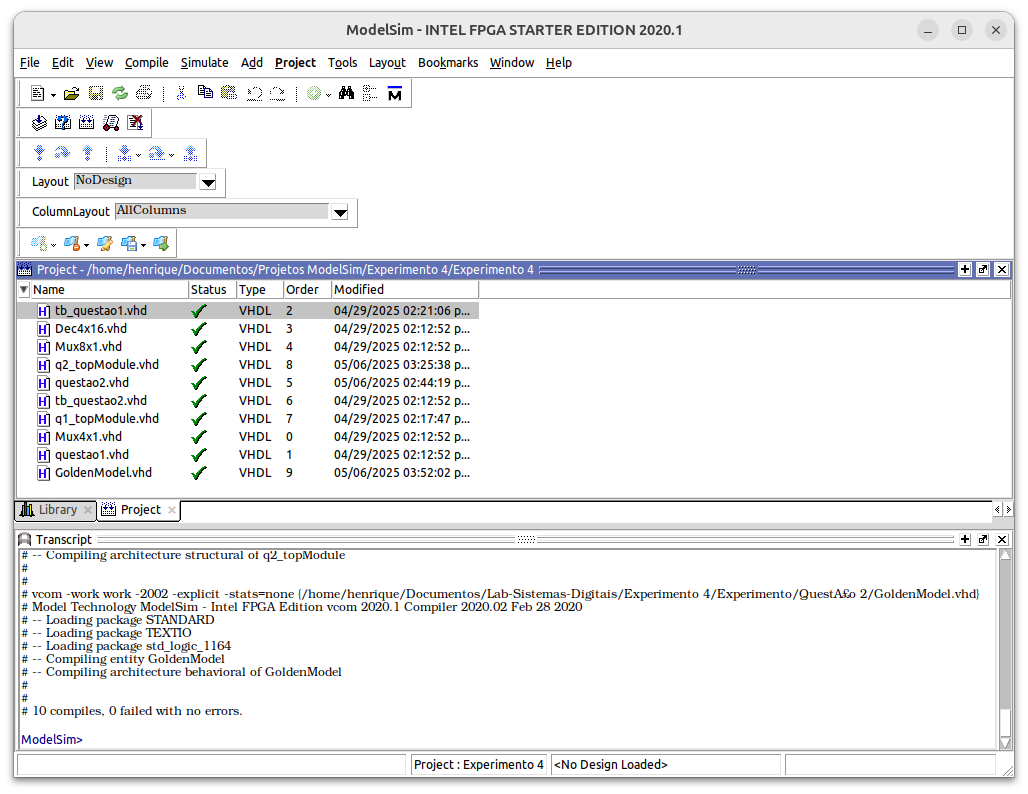
\includegraphics[width=1\textwidth]{Recursos/Imagens/CompileModelSim.png}
    \caption{Compilação de todos os códigos apresentados}
\end{figure}

\newpage

\section{Simulação}
O gráfico de forma de onda gerado pelo ModelSim ao simular o \textit{top-module} está exibido abaixo. Foram marcados com cursores os momento de interesse para a análise.

\begin{figure}[H]
    \centering
    \begin{tcolorbox}[colframe=cinza, colback=white, boxrule=0.75pt, arc=0pt, width=1\textwidth, center, boxsep=0pt, left=0pt, right=0pt, top=0pt, bottom=0pt]
    \includegraphics[width=1\textwidth]{Recursos/Imagens/wave.png}
    \end{tcolorbox}
    \caption{Simulação em forma de onda binária do moedeiro}
    \label{fig: ondas}
\end{figure}

\section{Análise}
Basta olhar o valor das saídas em \autoref{fig: ondas} que percebe-se o correto funcionamento do código apresentado. A saída $R$, de fato, é 1 apenas quando a máquina atinge ou ultrapassa R\$1,00 e as saídas $T_1$ e $T_0$ são ligadas apenas se o valor acumulado atinge R\$1,25 ou o cliente pede o dinheiro de volta (A = ``11'').

\section{Conclusão}
Nesse experimento, pela primeira vez, implementamos uma máquina de estados. Máquinas de estados são essenciais para a eletrônica digital; computadores nada mais são do que enormes associações de máquinas de estado de alta complexidade. A importância desse experimento reside nisso.

\end{document}